%\section{Implementation}
This chapter is dedicated to the implementation of the presented system. In this chapter we will explain in detail what has been implemented and how. 

\subsection{System}
%%In this section we will elaborate on the implementation for this project. We will delve into the system that the project is running on. We will shortly discuss the technological choices we have made and explain our reasons so.
%%%% Rasmus: Needs to be rewritten. Stupid. What do we want here?

\begin{figure}
	\centering
    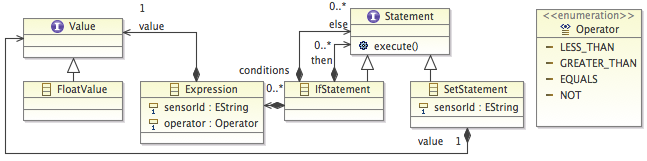
\includegraphics[scale=0.55]{chapters/implementation-model-expression-language.png} 
	\caption{The core classes in the \textit{expression language}.}
	\label{fig:ecore-sensors-actuators}
\end{figure}

A statement can either be a SetStatement or an IfStatement. The Set-statement sets an value in the simulator (in effect it is an actuator). It is possible to have nested If-statements, making the policies both flexible and simple. An If-statement can contain multiple expressions that all are being anded when evaluated. If the user wants to make an If-statement with or between the expressions, she will have to use a nested if. The optimal solution to this would have been to make a safe left-recursive model. We did not have enough time for this, but we will elaborate further on this subject in the \nameref{sec:discussion} section. An expression can contain the following operators; < > <= >= ! ==. 


\subsection{Interface Component}

\subsection{Abstraction Component}

\subsection{Storage Component}

\subsection{Request Flow}